%%This is a very basic article template.
%%There is just one section and two subsections.
\documentclass[a4paper, 11pt]{article}
\usepackage[pdftex]{graphicx}
\usepackage{parskip}
\usepackage{hyperref}
\usepackage[all]{hypcap}
\usepackage{amsmath}
\usepackage{amsfonts}
\usepackage{enumitem}
\usepackage{ tipa }
\title{Assignment 1 \\ MATH205: Linear Algebra}
\author{}

\newcommand{\mat}[1]{\boldsymbol { \mathsf{#1}} }

\begin{document}
\setlength{\parskip}{10pt}
\setlength{\parindent}{0pt}
\DeclareGraphicsExtensions{.pdf,.png,.gif,.jpg}
\maketitle

\section{Group Members}
\begin{enumerate}
	\item Muhammad Shahrom Ali
	\item Fizza Abbas 
	\item Muhammad Shahzain
\end{enumerate}

\newpage

\section{Questions}
\begin{enumerate}


\item Question 1

\begin{center}
  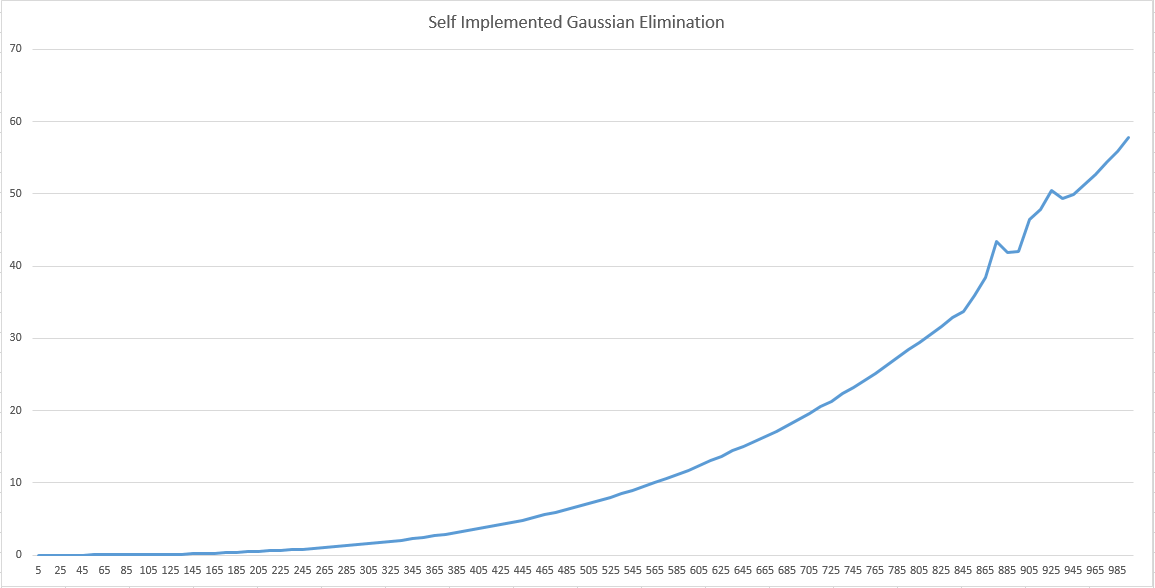
\includegraphics[width=\linewidth]{images/SelfImplemented.PNG}
\end{center}
Runtime of SelfImplemented Gaussian Elimination.

\begin{center}
  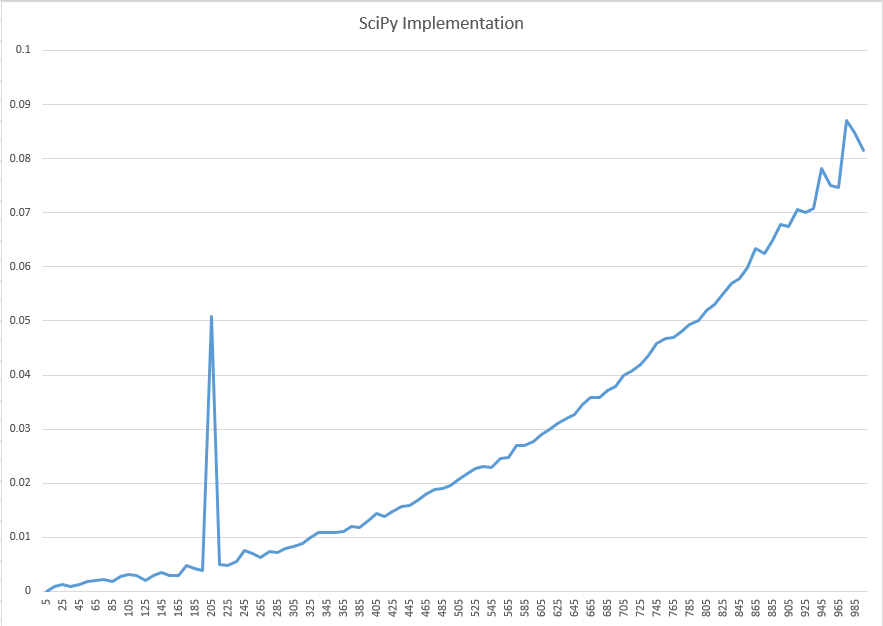
\includegraphics[width=\linewidth]{images/ScipyImplementation.PNG}
\end{center}
Runtime of SciPy Gaussian Elimination.


(Runtime on the vertical axes, matrix dimemsions on the horizontal axes)

As evident, the library implementation is much faster than our implementation of Gaussian Elimination. It takes less than 1 second for decomposition of a 985-matrix, compared to 58 seconds for our implementation. 

The curves are increasing exponentially though one thing that can be seen is that our curve increases much more smoothly as compared to the curve of scipy.

For Scipy,
205 seems to be an anomalous point in the running of the algorithm (perhaps due to the nature of the matrix?). We can also observe a few peaks near the end, and some more jerks throughout the curve which may be due to the heavy optimization in the library; there are some jerks and anomalies but the overall runtime is low.

For our implementaion, 
we can see that the runtime is sufficiently low for as large as 335-matrices (2.075451612 seconds) but, as observed earlier, runtime appears to be increasing exponentially and later the runtime increases by as much as 2 seconds (which is the total time for solving a 335-matrix) when increasing the dimensions of a matrix by 10.

Another important thing we can deduce is that the basic implementation of Gaussian elimination is good enough for small data sets of size 250 - 350. But it would be wiser to switch to the library implementation for any larger matrices. If the trends were drawn on the same graph, scipy would appear as a straight line.

(Python Code in Appendix \textbf{A}).
%

\item Question 2

The advantage given by LU factorization is that it decreases the overhead of calculations when Gaussian elimination is used to solve $k$ different systems of equations. For the below analysis, we have taken different sets of equations for each order (say 1x1, 2x2, …, 500x500). The code submitted (See Appendix \textbf{B}) will also show the differences in time complexities between the two methods of solving $k$ systems of equations.

The dataset (size, time) has been imported from the code, and has been used to plot respective scatter plots with polynomial fits, using MATLAB \cite{five}. The LU decomposition method shows a trend of $\mathcal{O}(n^3)$ while the Gaussian elimination with $k$ systems shows a higher trend ranging close to $\mathcal{O}(n^4)$.

We have set $k = \frac{n}{8}$ as we did not want $k$ to be too large. We know from the given question that the cost of solving systems of equations with LU decomposition is $\mathcal{O}(n^3 + kn^2)$ and on the other hand if we apply gaussian elimination, the runtime complexity of solving the system is $\mathcal{O}(kn^3)$. But since we have $k = \frac{n}{8}$, our equations eventually transform $\mathcal{O}(n^3 + n^{\frac{3}{8}}) = \mathcal{O}(n^3)$ and $\mathcal{O}(n^\frac{{4}{8}}) = \mathcal{O}(n^4)$, respectively.

The respective graphs are below:


\begin{center}
  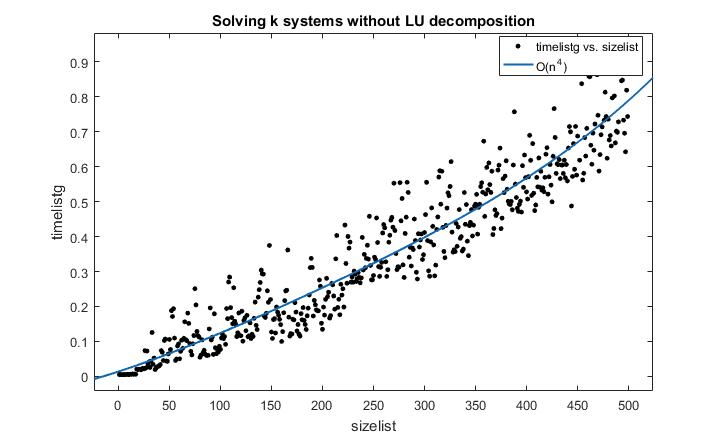
\includegraphics[width=\linewidth]{images/Gauss.jpg}
\end{center}

\begin{center}
  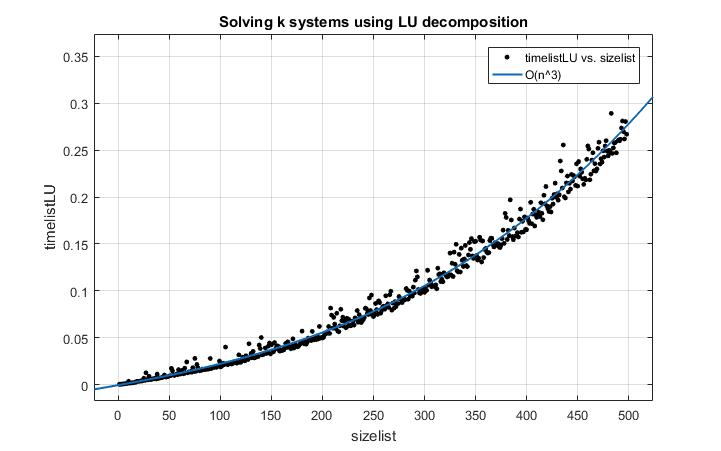
\includegraphics[width=\linewidth]{images/LU.jpg}
\end{center}


%
\item Question 3 
%

Linear combination is the sum of scaled vectors. 

If we have n vectors $\vec v_1, \vec v_2, \vec v_3, ..., \vec v_n$ and n scalars $a_1, a_2, a_3, ..., a_n$ then their linear combination can be written as: 

\begin{center}

$a_1\vec v_1 + a_2\vec v_2 + a_3\vec v_3 + ... + a_n\vec v_n$ 
\end{center}

where $\vec v_i$ is any arbitary vector of scalars, functions, polynomials, etc. and $a_i$ is a scalar which could be any non-zero number.

We call it a linear combination because if we put together two or more vectors in such a way that we fix the first vector and move the other vector(s) freely
in a way that they stay connected to one another then the resultant will always be a straight line (hence a \textit{linear} combination). Scaling any of the vectors
does not cause disconnection between the vectors hence we are allowed to scale the vectors and the summing of vectors is by the head-to-tale method; This is why we can scale the vectors and sum the vectors, resulting in the form mentioned above.

For example $\vec u = (2, 1)$ and $\vec v = (1, 1)$, and $\vec w = \vec u + \vec v$. This can be graphically represented as: 

\begin{center}
  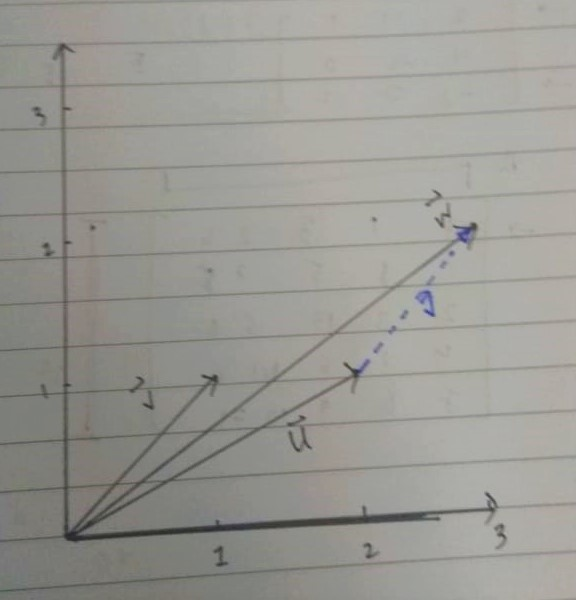
\includegraphics[width=\linewidth]{images/uvw.jpg}
\end{center}

$\vec w$ is the resultant vector and can be reached if we displace $\vec v$ to the head of $\vec u$ (blue dashed line).

We can say $\vec w$ is a linear combination of $\vec u$ and $\vec v$ with their scalars being 1.

Another example: $\vec x = \frac{1}{2}\vec u + \frac{1}{2}\vec v$

\begin{center}
  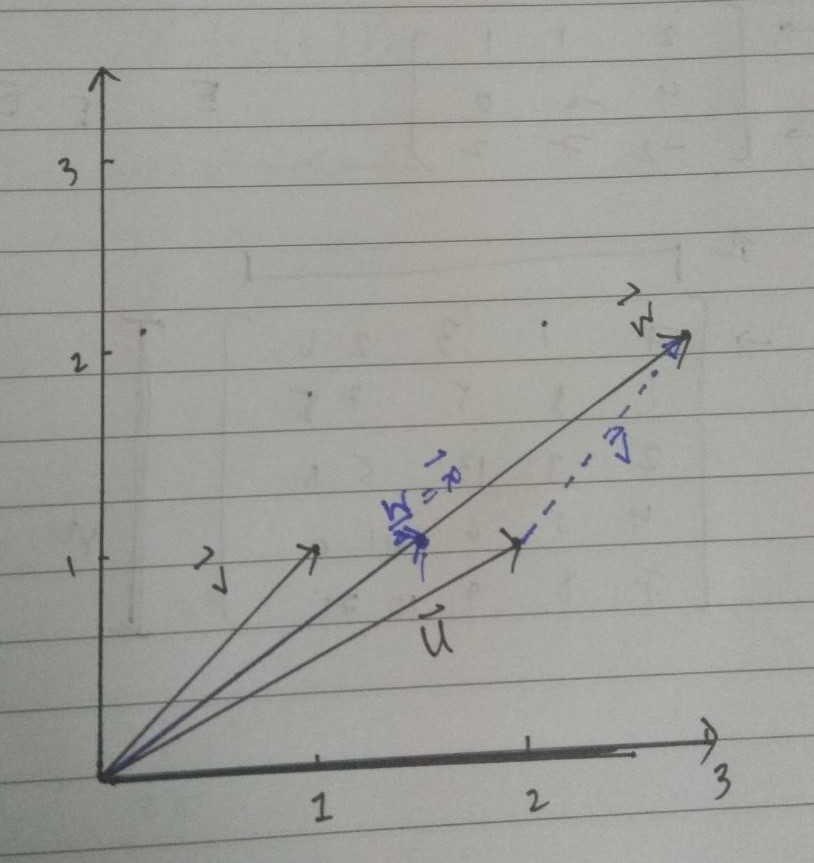
\includegraphics[width=\linewidth]{images/uvwx.jpg}
\end{center}

$\vec x = \frac{1}{2}(\vec u + \vec v)$

$\vec x = \frac{1}{2}\vec w$

And as represented in the graph above, the expression holds graphically aswell, with $\vec x$ being right up to the middle of $\vec w$.

For a systems of linear equations, 

\begin{center}
	$\vec a_1 + 2\vec a_2 = 4$ 

	$\vec a_1 + 4\vec a_2 = 10$
\end{center}  

	$\vec x = (1, 2)$

	$\vec y = (2, 4)$ 
	
	$\vec r = (4, 10)$

	The above equation shows how many of $\vec a_1$ and $\vec a_2$ is required to make the resultant $\vec r$.

	This can be shown as
	
	$a_1 
	\begin{bmatrix} 
		1 \\ 
		2 
	\end{bmatrix}
	+ a_2
	\begin{bmatrix}
	2 \\
	4
	\end{bmatrix}
	= 
	\begin{bmatrix}
	4 \\
	10
	\end{bmatrix}
	$
	
	The equations are solved simultaneously to find the values of $a_1$ and $a_2$.
	Upon solving:
	\begin{center}
	$0 = -2$
	\end{center}
	This represents that there is no linear combination of these vectors possible. Graphically, it means that the lines do not 
	intersect at any point i.e. they are parallel to each other as shown in figure below:

	\begin{center}
  	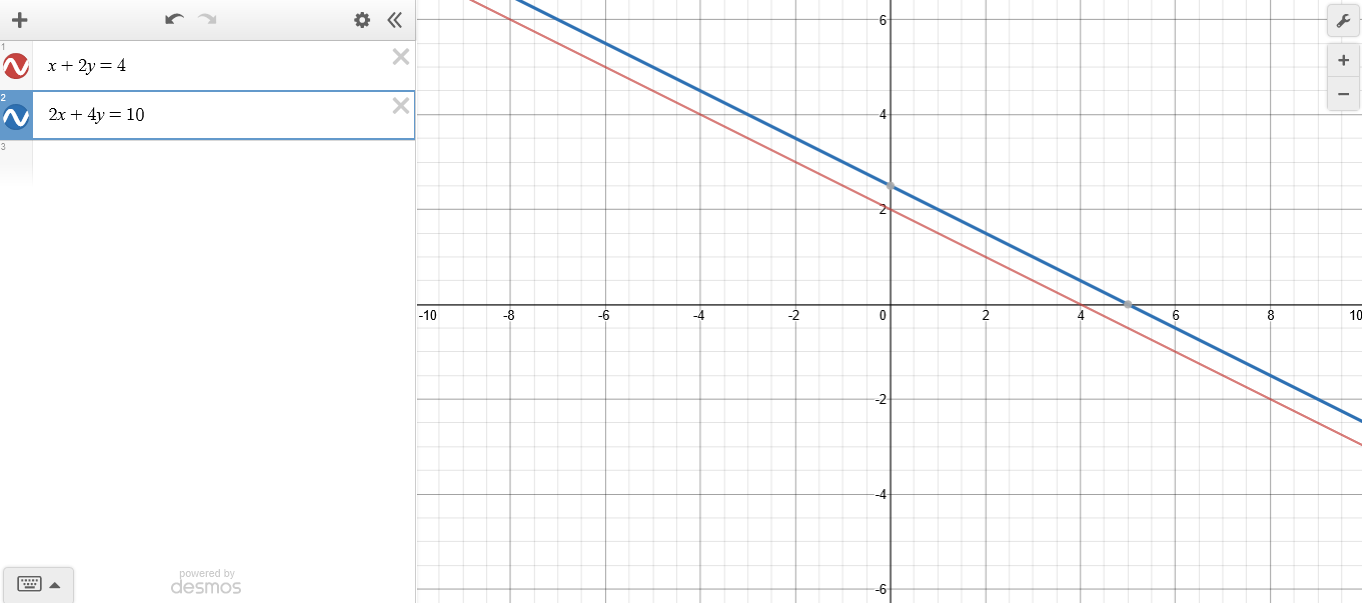
\includegraphics[width=\linewidth]{images/no solution line.PNG}
	\end{center}

	Another system of linear equations,
	
	\begin{center}
	$\vec a_1 + 2\vec a_2 = 4$ 

	$\vec a_1 + 4\vec a_2 = 8$
	\end{center}  
	
	
	Upon solving:
	\begin{center}
		$0 = 0$
	\end{center}
	
	This represents that there are infinite linear combinations possible for the above equations. Graphically, It means that the two lines intersect at every point i.e. they are collinear as shown in figure below:
	
	\begin{center}
  	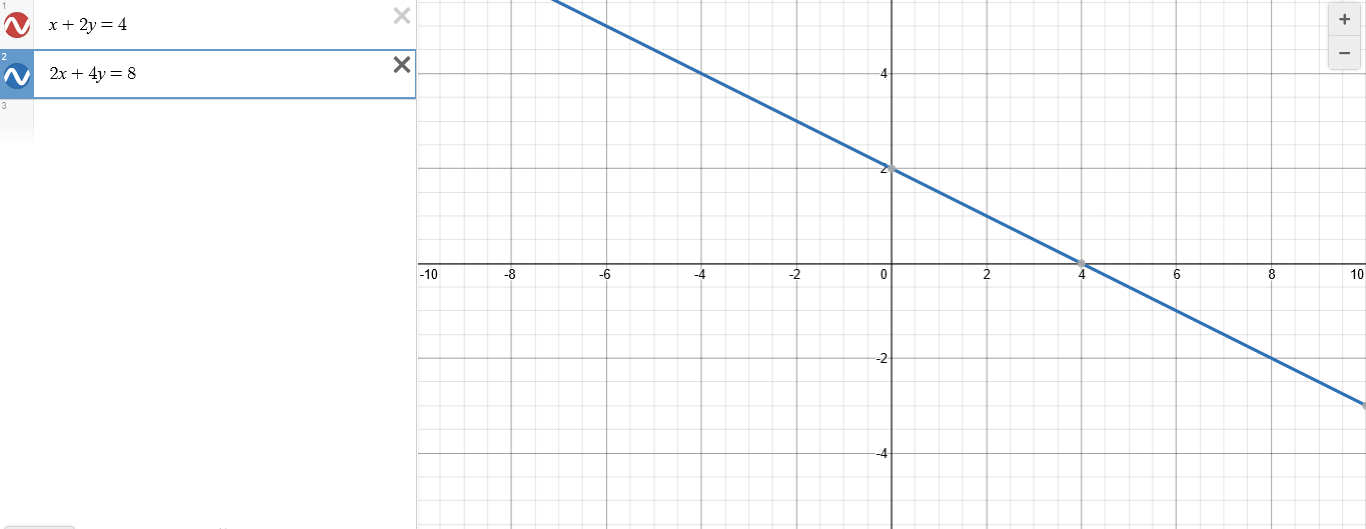
\includegraphics[width=\linewidth]{images/infinitely_many_solutions.PNG}
	\end{center}

	Consider another system of linear equations.

	\begin{center}
	$3\vec a_1 + 4\vec a_2 = 10$ 

	$2\vec a_1 + 4\vec a_2 = 4$
	\end{center}  	
	
	Upon solving 
	\begin{center}
		$a_1 = 6; a_2 = -2$
	\end{center}
	
	This represents that a unique linear combination of vectors 
	$ \begin{bmatrix} 
		3 \\ 
		4
	\end{bmatrix}$
	and vector  
	$ \begin{bmatrix} 
		4 \\ 
		4 
	\end{bmatrix}$
	 to give a resultant vector
	 $ \begin{bmatrix} 
		10 \\ 
		4 
	\end{bmatrix}$.
	Graphically, the two lines intersect at only one point, as shown in the figure below:
	
	\begin{center}
  	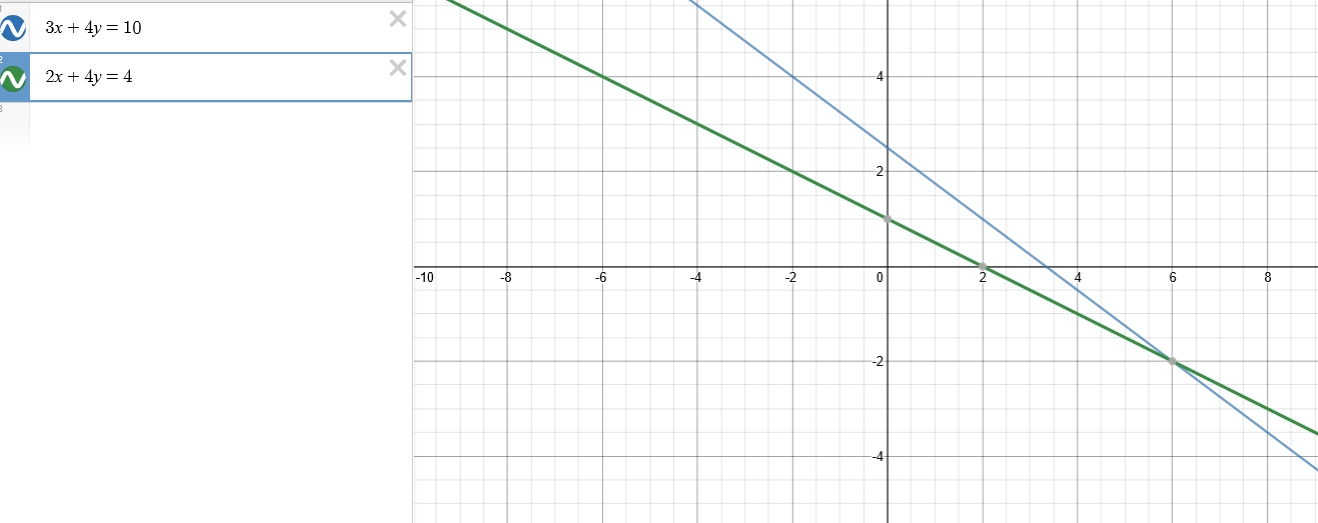
\includegraphics[width=\linewidth]{images/unique_solution.PNG}
	\end{center}
	
	Just as we discussed lines in $\mathcal{R}^2$ we discuss planes in $\mathcal{R}^3$. 

	If we have vectors in the form,

	$ 
	a_1\begin{bmatrix} 
		x_1 \\ 
		x_2 \\
		x_3
	\end{bmatrix}
	+ 
	a_2\begin{bmatrix} 
		y_1 \\ 
		y_2 \\
		y_3
	\end{bmatrix}
	+
	a_3\begin{bmatrix} 
		z_1 \\ 
		z_2 \\
		z_3
	\end{bmatrix}
	$
	
	then their linear combination will only be possible if all these planes intersect.
 	
 	If the planes intersect at just one common point then they have a unique solution. This is shown in figure below.  \cite{three}
 	
 	\begin{center}
  	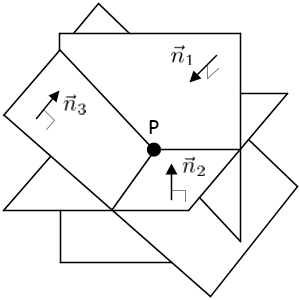
\includegraphics[width=\linewidth]{images/unique_solution_plane.png}
	\end{center}
 	
If the planes intersect such that the intersection is not a point but a line then there are infinitely many linear combinations possible. This is shown in figure below. \cite{six}
	
	 	\begin{center}
  	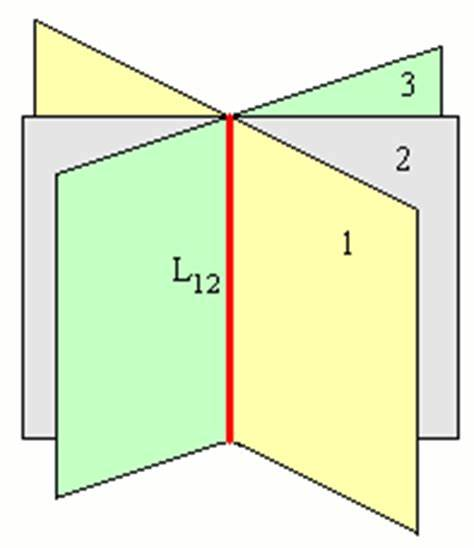
\includegraphics[width=\linewidth]{images/infinite_solutions_plane.jpg}
	\end{center}
	
	If all the planes do not meet at some point together (For example, if out of 4 planes two intersect at one point and the other two intersect at some other point) then the linear combination of these planes is not possible.  This is shown in figure below. \cite{seven} \cite{eight}
	
	\begin{center}
		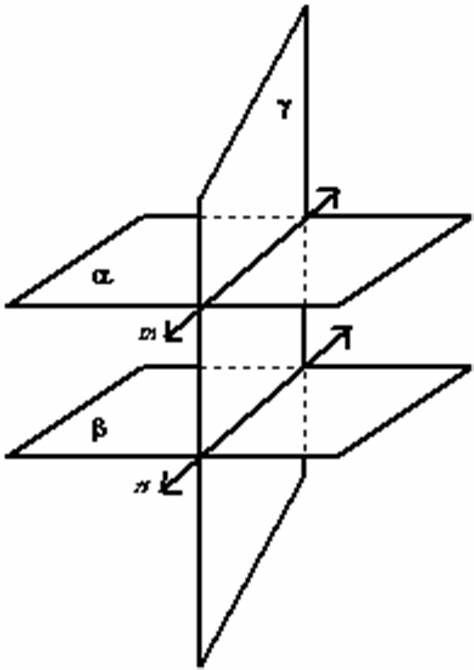
\includegraphics[width=\linewidth]{images/no_solution_plane_2.jpg}
	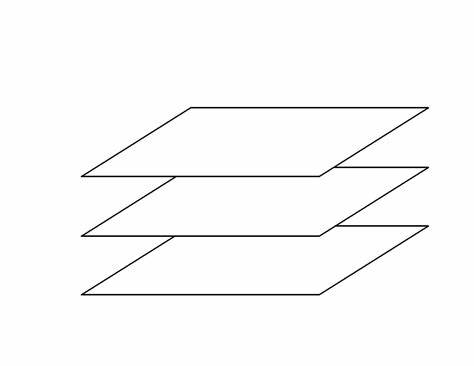
\includegraphics[width=\linewidth]{images/no_solution_plane.jpg}
\end{center}•


\item Question 4
\begin{enumerate}[label=(\alph*)]

\item Gaussian elimination can be done as a series of matrix multiplications with $\mat{A}$ resulting in an upper-triangular matrix $\mat{U}$. 

To convert this into an upper triangular matrix $\mat{U}$, we need to convert entries $\mat{A}_{21}$, $\mat{A}_{31}$, and $\mat{A}_{41}$ to 0.

$-\frac{v_2}{v_1}$\textscr$_1$ + \textscr$_2$

$\mat{E}_{21} = $
$\begin{bmatrix} 
       1 & 0 & 0 & 0 \\ 
       -\frac{v_2}{v_1} & 1 & 0 & 0 \\
       0 & 0 & 1 & 0 \\
       0 & 0 & 0 & 1 
\end{bmatrix}$

$-\frac{v_3}{v_1}$\textscr$_1$ + \textscr$_3$

$\mat{E}_{31} = $
$\begin{bmatrix} 
       1 & 0 & 0 & 0 \\ 
       0 & 1 & 0 & 0 \\
       -\frac{v_3}{v_1} & 0 & 1 & 0 \\
       0 & 0 & 0 & 1 
\end{bmatrix}$

$-\frac{v_4}{v_1}$\textscr$_1$ + \textscr$_4$

$\mat{E}_{41} = $
$\begin{bmatrix} 
       1 & 0 & 0 & 0 \\ 
       0 & 1 & 0 & 0 \\
       0 & 0 & 1 & 0 \\
       -\frac{v_4}{v_1} & 0 & 0 & 1
\end{bmatrix}$

$\mat{E}_{41}\mat{E}_{31}\mat{E}_{21}\mat{A} = \mat{U}$

We can write this as $\mat{E}\mat{A} = \mat{U}$ 

$\mat{E} = \mat{E}_{41}\mat{E}_{31}\mat{E}_{21} = $
$\begin{bmatrix} 
       1 & 0 & 0 & 0 \\ 
       -\frac{v_2}{v_1} & 1 & 0 & 0 \\
       -\frac{v_3}{v_1} & 0 & 1 & 0 \\
       -\frac{v_4}{v_1} & 0 & 0 & 1 
\end{bmatrix}$

$\mat{E}\mat{A} = \mat{U} = $
$\begin{bmatrix} 
       v_1 & 0 & 0 & 0 \\ 
       0 & 1 & 0 & 0 \\
       0 & 0 & 1 & 0 \\
       0 & 0 & 0 & 1 
\end{bmatrix}$

We can also say $\mat{A} = \mat{E}^{-1}\mat{U}$ where, $\mat{E}^{-1}$ is a lower triangular matrix so it can be called $\mat{E}^{-1} = \mat{L}$ so

$\mat{A} = \mat{L}\mat{U}$

$\mat{L} = \mat{E}^{-1} = $
$\begin{bmatrix} 
       1 & 0 & 0 & 0 \\ 
       \frac{v_2}{v_1} & 1 & 0 & 0 \\
       \frac{v_3}{v_1} & 0 & 1 & 0 \\
       \frac{v_4}{v_1} & 0 & 0 & 1 
\end{bmatrix}$

$\mat{A} = \mat{L}\mat{U} = $
$\begin{bmatrix}
		1 & 0 & 0 & 0 \\ 
       \frac{v_2}{v_1} & 1 & 0 & 0 \\
       \frac{v_3}{v_1} & 0 & 1 & 0 \\
       \frac{v_4}{v_1} & 0 & 0 & 1 
\end{bmatrix}
\begin{bmatrix} 
       v_1 & 0 & 0 & 0 \\ 
       0 & 1 & 0 & 0 \\
       0 & 0 & 1 & 0 \\
       0 & 0 & 0 & 1 
\end{bmatrix}$

\item $\mat{A} = \mat{LU}$

$\mat{A^{-1}} = (\mat{LU})^{-1}$

$\mat{A^{-1}} = \mat{U^{-1}L^{-1}}$

From the previous part we know, $\mat{L^{-1}} = \mat{E}$ hence

$\mat{A^{-1}} = \mat{U^{-1}E}$

Since $\mat{U}$ is a diagonal matrix, $\mat{U}^{-1}$ =
$\begin{bmatrix} 
       \frac{1}{v_1} & 0 & 0 & 0 \\ 
       0 & 1 & 0 & 0 \\
       0 & 0 & 1 & 0 \\
       0 & 0 & 0 & 1 
\end{bmatrix}$ 

and $\mat{E} = $
$\begin{bmatrix} 
       1 & 0 & 0 & 0 \\ 
       -\frac{v_2}{v_1} & 1 & 0 & 0 \\
       -\frac{v_3}{v_1} & 0 & 1 & 0 \\
       -\frac{v_4}{v_1} & 0 & 0 & 1 
\end{bmatrix}$

$\mat{A}^{-1} = $
$\begin{bmatrix} 
       \frac{1}{v_1} & 0 & 0 & 0 \\ 
       0 & 1 & 0 & 0 \\
       0 & 0 & 1 & 0 \\
       0 & 0 & 0 & 1 
\end{bmatrix}$ 
$\begin{bmatrix} 
       1 & 0 & 0 & 0 \\ 
       -\frac{v_2}{v_1} & 1 & 0 & 0 \\
       -\frac{v_3}{v_1} & 0 & 1 & 0 \\
       -\frac{v_4}{v_1} & 0 & 0 & 1 
\end{bmatrix}$

$\mat{A}^{-1} = $
$\begin{bmatrix} 
        \frac{1}{v_1} & 0 & 0 & 0 \\ 
       -\frac{v_2}{v_1} & 1 & 0 & 0 \\
       -\frac{v_3}{v_1} & 0 & 1 & 0 \\
       -\frac{v_4}{v_1} & 0 & 0 & 1 
\end{bmatrix}$


\item For any non-singular matrix $\mat{A}$ there exists one and only one matrix $\mat{A}^{-1}$ such that $\mat{AA}^{-1} = \mat{I}.$ \cite{one}

If $\mat{A} = \mat{L}_{1}\mat{U}_{1}$ and $\mat{A} = \mat{L}_{2}\mat{U}_{2}$ 

then $\mat{A}^{-1} = \mat{U}_1^{-1}\mat{L}_1^{-1}$ and $\mat{A}^{-1} = \mat{U}_2^{-1}\mat{L}_2^{-1}$ 

$\mat{AA}^{-1} = \mat{L}_{1}\mat{U}_{1}\mat{A}^{-1}$

$\mat{AA}^{-1} = \mat{L}_{1}\mat{U}_{1}\mat{U}_2^{-1}\mat{L}_2^{-1}$

$\mat{I} =  \mat{L}_{1}\mat{U}_{1}\mat{U}_2^{-1}\mat{L}_2^{-1}$

and the only way for $\mat{L}_{1}\mat{U}_{1}\mat{U}_2^{-1}\mat{L}_2^{-1} = \mat{I}$ is if $\mat U_2^{-1} = \mat U_1^{-1}$ and $\mat L_2^{-1} = \mat L_1^{-1}$ which is only possible if $\mat U_1 = \mat U_2$ and $\mat L_1 = \mat L_2.$

Furthermore if $\mat{A} = \mat{L}_{1}\mat{U}_{1}$ and $\mat{A} = \mat{L}_{2}\mat{U}_{2}$ then since matrix multiplication is not commutative, if $\mat{L}_1\mat{U}_1 = \mat{L}_2\mat{U}_2$ then $\mat{L}_1$ must $= \mat{L}_2$ and $\mat{U}_1$ must $= \mat{U}_2$.

\item LU decomposition of \textbf{any} matrix $\mat A$ can also be written as $\mat A = \mat {LDU}$ where $\mat L$ and $\mat U$ are lower and upper triangular matrices, respectively with 1s as their pivots, and $\mat D$ is a diagonal matrix. 

For any arbitrary non-singular matrix $\mat A$: 

$\mat A = \mat{LDU}$ and $\mat A^T = (\mat{LDU})^T$

When $\mat A$ is a symmetric matrix, we know that $\mat A = \mat A^T$

$\mat A = \mat{LDU} = \mat A^T = (\mat{LDU})^T$

$\mat{LDU} = \mat U^T \mat D^T \mat L^T$

$\mat D $ is a diagonal matrix hence the transpose of it is the same.

$\mat{LDU} = \mat U^T \mat D \mat L^T$

Since matrix multiplication is not commutative, for the equality to hold, $\mat L = \mat U^T$ and $\mat U = \mat L^T$

$\mat A^T = \mat U^T \mat D \mat L^T = \mat A$

$\mat A = \mat U^T \mat D \mat L^T$ and since $\mat L = \mat U^T$ , 

$\mat A = \mat L \mat D \mat L^T$

\end{enumerate}
\end{enumerate}

\newpage

\section{Appendix A}
Python Code for Question 1. \cite{two}
	\begin{verbatim}
import random, time
from scipy.linalg import lu

#implement a basic GE algorithm and compare it's runtime 
#with that of a library implementation

#elementary row operations
def row_mul(s, lst):
    return [i*s for i in lst]

def row_subt(r2, r1):
    #r2 - r1
    #r1 and r2 are a row of the matrix (in a list)
    assert len(r1) == len(r2)
    return [r2[i] - r1[i] for i in range(len(r1))]

#Gaussian Elimination implementation:
def GE(mat):
    for i in range(1, len(mat)):
        for j in range(i):
            if mat[j][j] == 0:
                return False
            mat[i] = row_subt(mat[i], row_mul(mat[i][j]/mat[j][j], mat[j])) 
    return mat

def generateMatrix(dim):
    return [[random.randint(1, 10) for i in range(dim)] for j in range(dim)]

def main():

    record = open("SelfImplementedGE.csv", "w")
    scipyRecord = open("SciPyGE.csv", "w")

    for i in range(5, 500, 5):
			
        A = generateMatrix(i) #Matrix for Self Implemented GE
        B = [i.copy() for i in A]

        start_time = time.time()
		
        while GE(A) == False: #if A is singular
            A = generateMatrix(i) #Regenerate a matrix 
            B = [i.copy() for i in A] 
            start_time = time.time() #restart timer

        stop_time = time.time() - start_time
		
        record.write(str(i) + ", " + str(stop_time) + "\n")
		
        start_time = time.time()
		
        pl, u = lu(B, permute_l=True)
		
        stop_time = time.time() - start_time
		
        scipyRecord.write(str(i) + ", " + str(stop_time) + "\n")
		
		
    record.close()
    scipyRecord.close()

main()

	\end{verbatim}


\newpage

\section{Appendix B}
Python Code for Question 2

\begin{verbatim}
import numpy as np
import scipy
import scipy.linalg
import time
import matplotlib.pyplot as plt

def create_square_matrix(_type,order):
    if _type == 1:
        return scipy.random.randint(1,200,(order,order))
    if _type == 2:
        return numpy.random.randint(1,200,(order,order))
    
timeListLU=[]
sizeListLU=[]
timeListG=[]
def makeGraph(n):
    
    for i in range(8,n,1):
        A = create_square_matrix(1,i)
        a=time.clock()
        LU = scipy.linalg.lu_factor(A)
        for j in range (i):
            b=scipy.random.randint(1,20,(i,1))
            result=scipy.linalg.lu_solve(LU,b)   
        b=time.clock()
        
        sizeListLU.append(i)
        print(i)
        timeListLU.append(b-a)
        a=time.clock()
        for j in range (i//8):
            b=scipy.random.randint(1,20,(i,1))
            result=np.linalg.solve(A,b)
        b=time.clock()
        timeListG.append(b-a)
    plt.plot(sizeListLU,timeListG)
    plt.plot(sizeListLU,timeListLU)
    
    ## plt.plot(sizeListLU,[(a*i)**3 for i in sizeListLU])
    plt.show()


makeGraph(200)
\end{verbatim}

\newpage

\begin{thebibliography}{9}
        \bibitem{one}
		Dr. Majeed's lecture notes. 
		\\ \textit{Lecture 4 slide 5/23: Existence of an inverse}

       \bibitem{two}
              Using Scipy for LU Decomposition
	   \begin{verbatim}
https://stackoverflow.com/questions/15638650/is-there-a-
standard-solution-for-gauss-elimination-in-python
		\end{verbatim}
       \bibitem{three}
       		Planes intersecting at one point
       		\begin{verbatim}
https://www.bing.com/th?id=OIP.9YOKRzWPzMUt5CjadfiBDAAAAA&pid=Api&rs=1
\end{verbatim}
       		
       \bibitem{four}
       		Desmos for plotting lines (Question 1)
        
        \bibitem{five}
        		Mathworks: MATLAB for Question 2
        
        \bibitem{six}
       		Planes intersecting on a line.
       		\begin{verbatim}
		https://www.bing.com/th?id=OIP._tToqHdNhT-VvimtTnFngQHaIk&pid=Api&rs=1
		\end{verbatim}
	
	\bibitem{seven}
       		Planes not intersecting 1
       		\begin{verbatim}
			https://www.bing.com/th?id=OIP.hMuQlz6JpsSQKbXlhdVwoAHaKe&pid=Api&rs=1
		\end{verbatim}

	\bibitem{eight}
       		Planes not intersecting 2
       		\begin{verbatim}
		https://www.bing.com/th?id=OIP.0UYCquCiPyS3dLcd8KWVOQHaFu&pid=Api&rs=1
		\end{verbatim}

\end{thebibliography}
\end{document}